\documentclass[
  english,
  aspectratio=169,
  sectionpage=false,
]{tumbeamer}

\usepackage{graphicx}
\usepackage{booktabs}
\usepackage{tikz}
\usetikzlibrary{arrows.meta,positioning,fit,backgrounds}

\title{Dollhouse}
\subtitle{Progress Update \#1}
\author{Leonhard Driesch}
\institute{Visual Computing \& Artificial Intelligence\\Prof.\ Matthias Nie\ss{}ner\\Technical University of Munich}
\date[09/23/2026]{September 23\textsuperscript{rd}, 2026}

\footline{\insertauthor~|~\insertshorttitle~|~\insertshortdate}

\TUMbeamersetup{
  title page = TUM tower,
  part page = TUM toc,
  section page = TUM toc,
  content page = TUM more space,
  tower scale = 1.0,
  headline = TUM threeliner,
  footline = TUM default,
  headline on = {title page},
  footline on = {every page, title page=false},
}

\tikzset{
  box/.style={
    rounded corners=2pt,
    draw=TUMBlue,
    fill=TUMBlue!8,
    align=center,
    font=\small
  },
  ghost/.style={
    box,
    draw=TUMGray,
    fill=TUMGray!12
  },
  flow/.style={-{Latex[length=2.2mm]}, very thick, draw=TUMBlue},
  weakflow/.style={-{Latex[length=2.2mm]}, thick, draw=TUMGray},
}

\newcommand{\legendcol}[3]{%
  \begin{column}{#1}
    \footnotesize
    \textbf{#2}\par#3
  \end{column}}

\begin{document}

\maketitle

\begin{frame}{Pipeline}
  \centering
  \vfill
  \begin{tikzpicture}[node distance=8mm]
    \node[ghost, text width=2.8cm, minimum height=14mm] (det)
      {Detection\\[2pt]\scriptsize model open};
    \node[box, text width=2.8cm, minimum height=14mm, right=of det] (ext)
      {Image extraction\\[2pt]\scriptsize Qwen-Image 2.1};
    \node[box, text width=2.8cm, minimum height=14mm, right=of ext] (i23d)
      {Image-to-3D\\[2pt]\scriptsize TRELLIS.2};
    \node[ghost, text width=2.8cm, minimum height=14mm, right=of i23d] (asm)
      {Scene assembly\\[2pt]\scriptsize method open};

    \draw[flow] (det) -- (ext);
    \draw[flow] (ext) -- (i23d);
    \draw[flow] (i23d) -- (asm);
  \end{tikzpicture}
  \vfill
\end{frame}

\begin{frame}
  \centering
  \vfill
  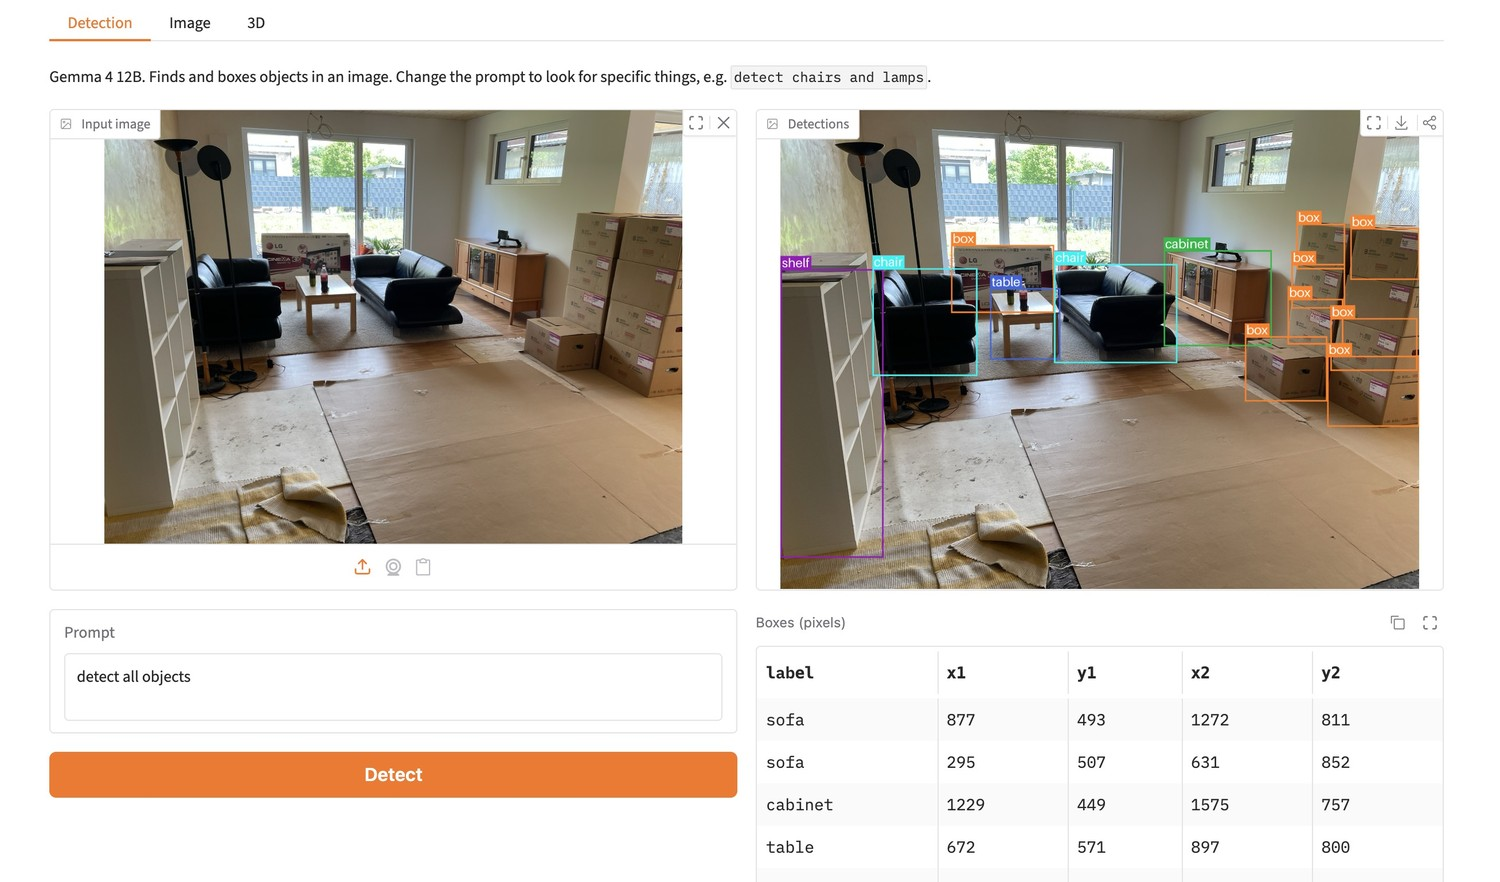
\includegraphics[width=\linewidth,height=0.9\textheight,keepaspectratio]{figures/detection.jpg}
  \vfill
\end{frame}

\begin{frame}{Detection: which model?}{Find every object in a room photo, no fixed class list}
  \begin{columns}[T,onlytextwidth]
    \begin{column}{0.47\textwidth}
      \textbf{VLM} \hfill {\footnotesize\color{TUMGray} current attempt}\par
      \vspace{2mm}
      \footnotesize
      Gemma 4 12B, prompt ``detect all objects'', boxes parsed from the text output.
      \begin{itemize}\footnotesize
        \item[+] Free-form prompt; can decide what counts as an object
        \item[--] Boxes come from generated text
        \item[--] Large (12B) and slow
      \end{itemize}
    \end{column}
    \begin{column}{0.47\textwidth}
      \textbf{Open-vocabulary detector}\par
      \vspace{2mm}
      \footnotesize
      Grounding DINO, OWLv2, YOLO-World, SAM~3, \ldots
      \begin{itemize}\footnotesize
        \item[+] Trained for localization; masks with SAM~3
        \item[+] Small and fast
        \item[--] Needs the class names as text input
      \end{itemize}
    \end{column}
  \end{columns}

  \vfill
  \begin{center}
    \begin{tikzpicture}
      \node[box, text width=0.8\textwidth, inner sep=2mm, font=\small]
        {VLM, detector, or both (VLM names the objects, detector localizes them)?\\[2pt]
         \footnotesize Other models for this use case?};
    \end{tikzpicture}
  \end{center}
\end{frame}

\begin{frame}
  \centering
  \vfill
  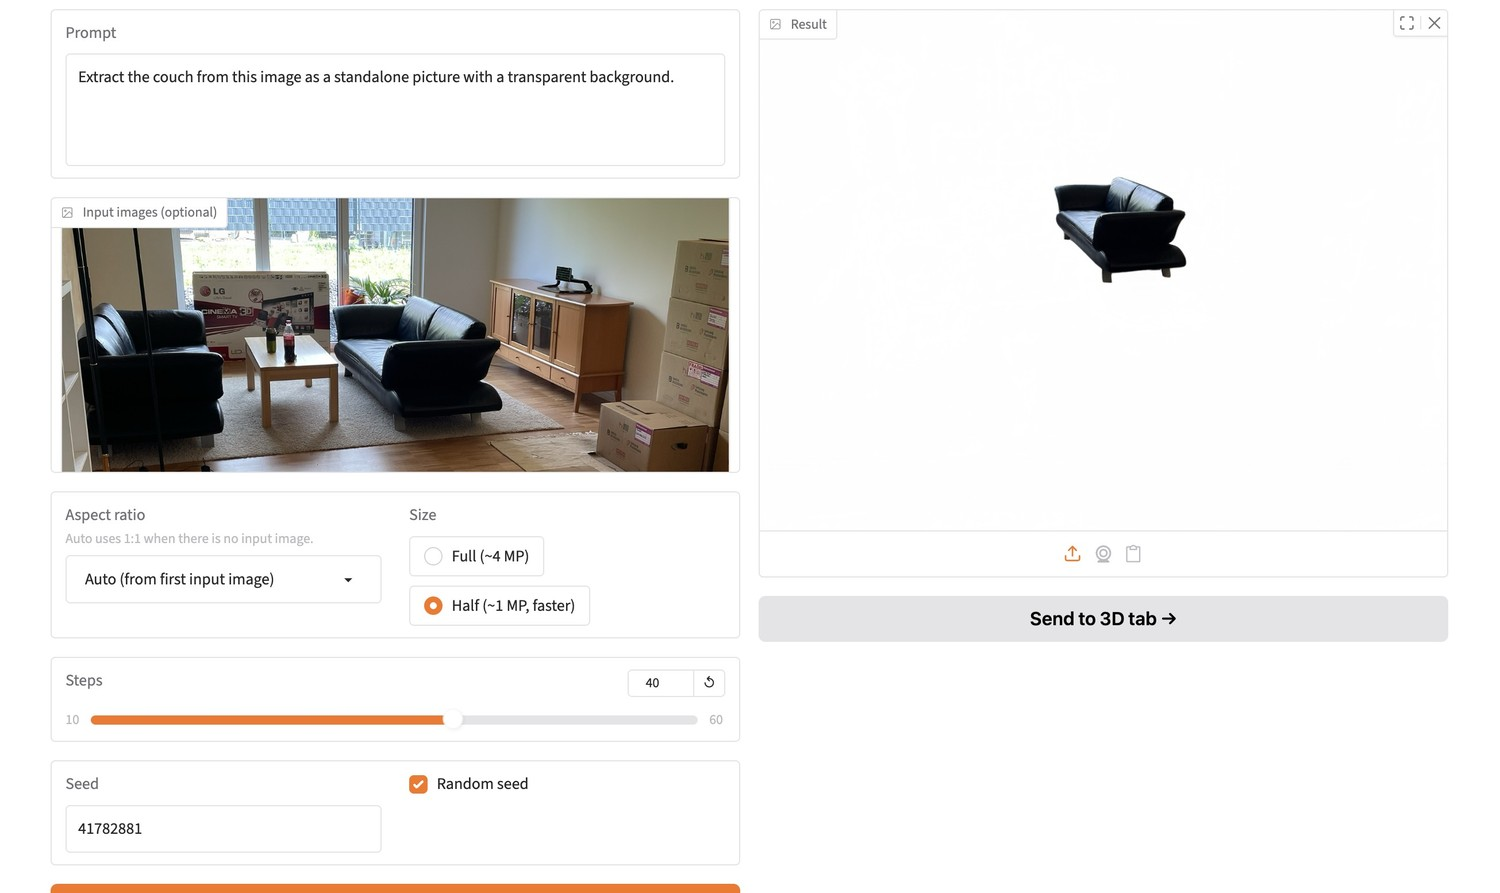
\includegraphics[width=\linewidth,height=0.9\textheight,keepaspectratio]{figures/image-extraction.jpg}
  \vfill
\end{frame}

\begin{frame}
  \centering
  \vfill
  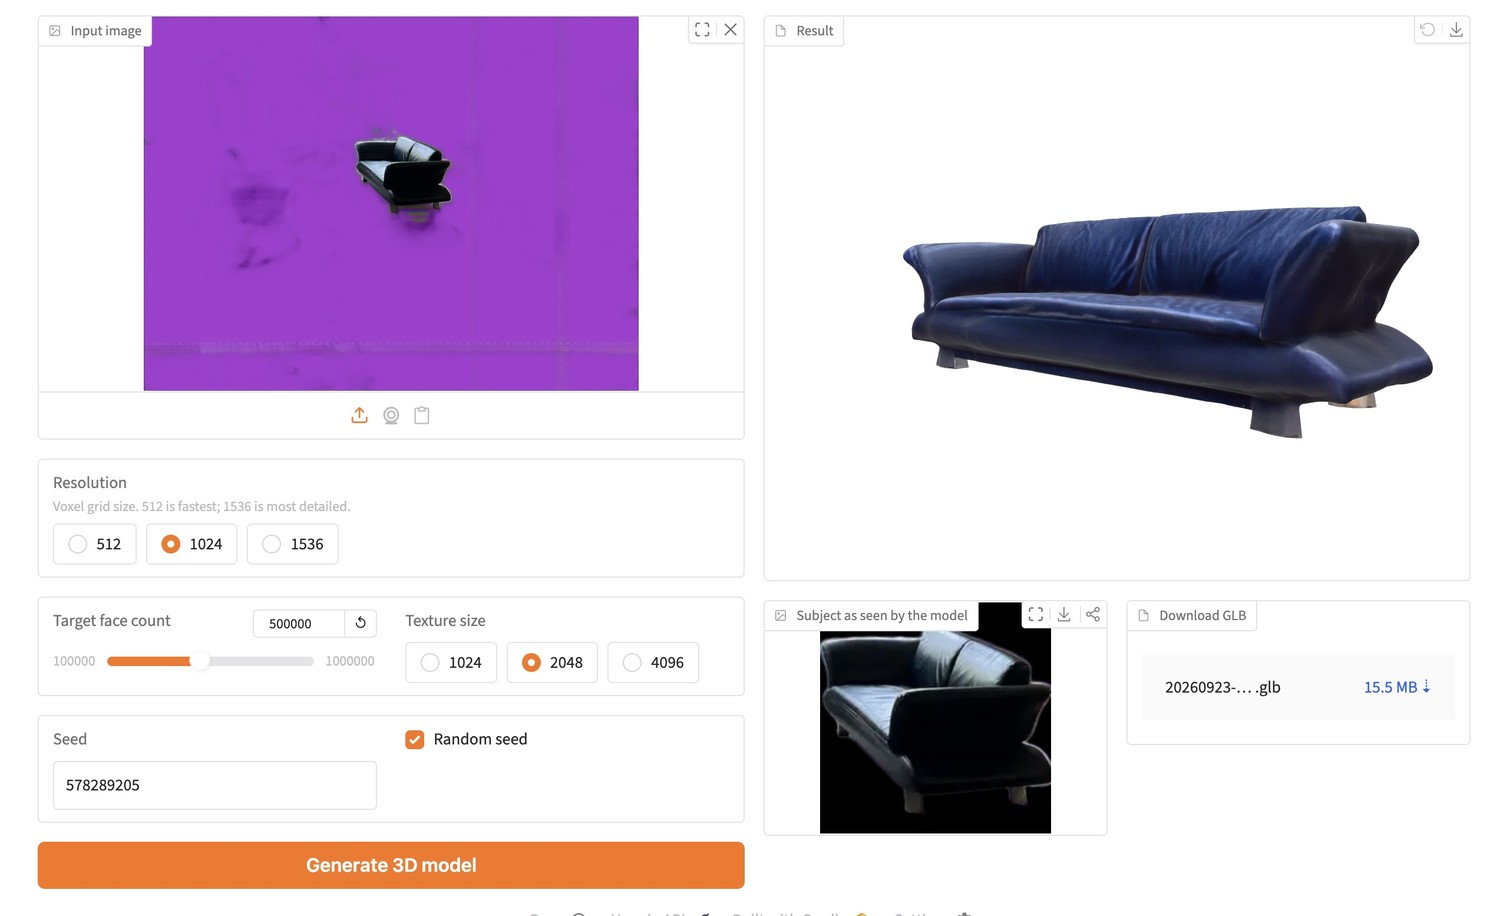
\includegraphics[width=\linewidth,height=0.9\textheight,keepaspectratio]{figures/image-to-3d.jpg}
  \vfill
\end{frame}

\begin{frame}
  \centering
  \vfill
  \begin{columns}[T,onlytextwidth]
    \begin{column}{0.49\textwidth}
      \centering
      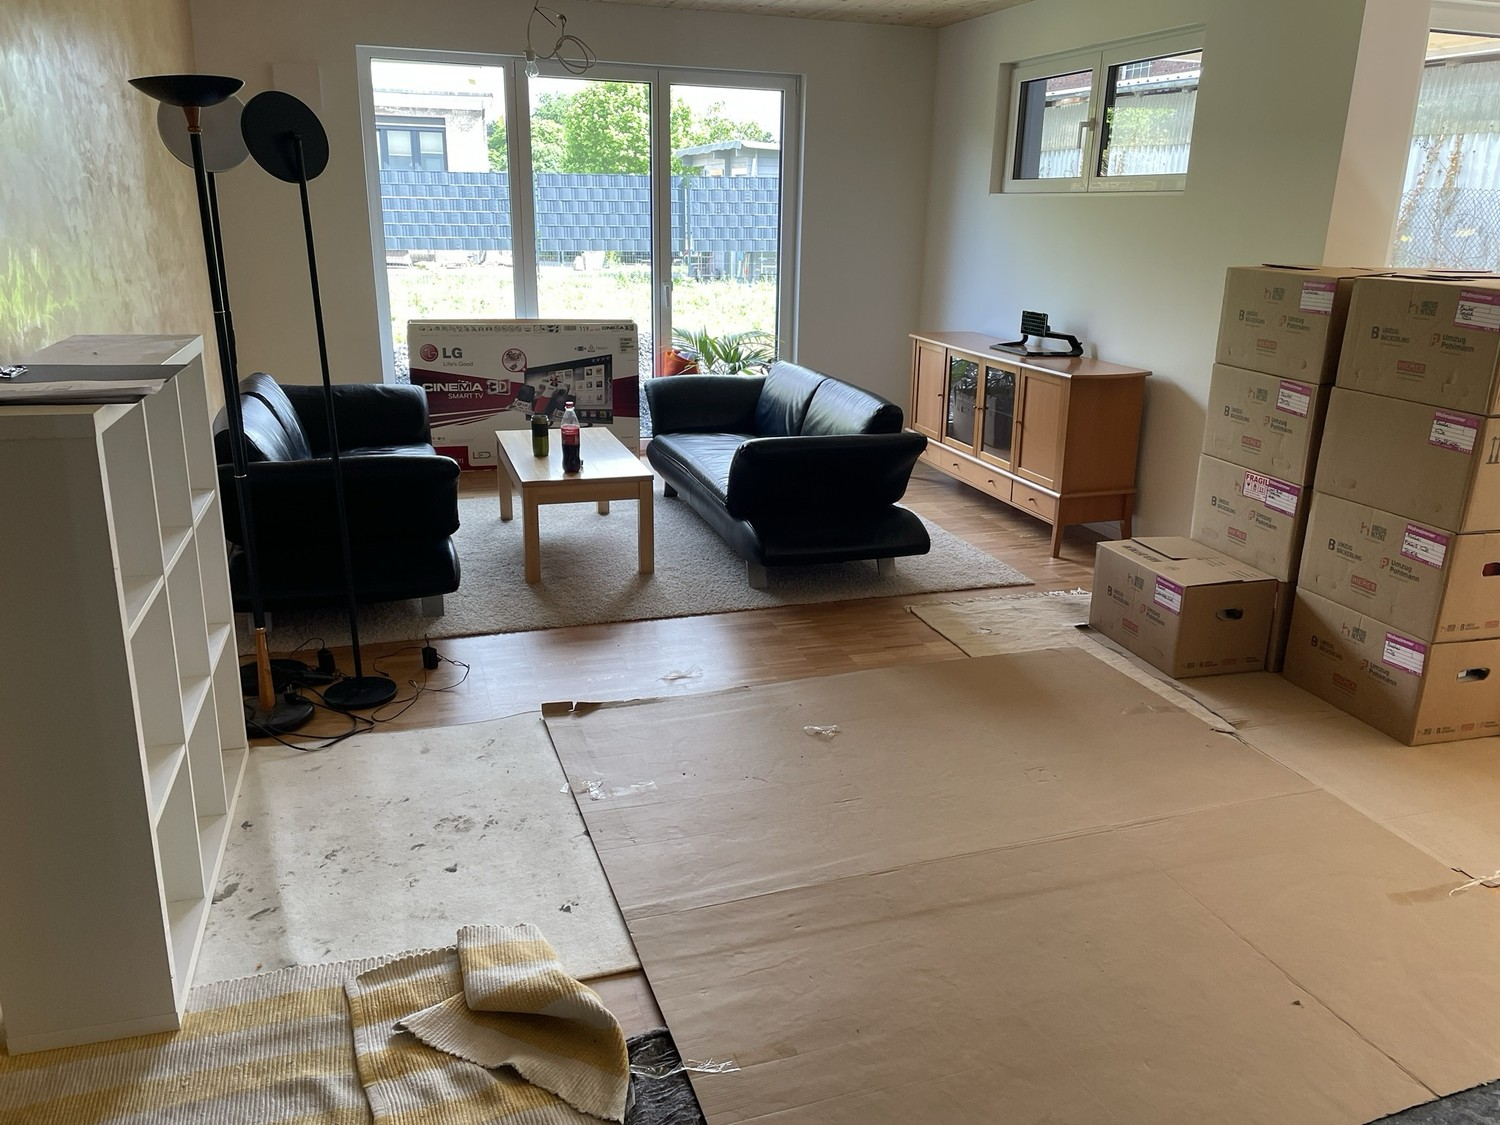
\includegraphics[width=\linewidth]{figures/original-photo.jpg}\par
      \vspace{2mm}
      {\footnotesize Original photo}
    \end{column}
    \begin{column}{0.49\textwidth}
      \centering
      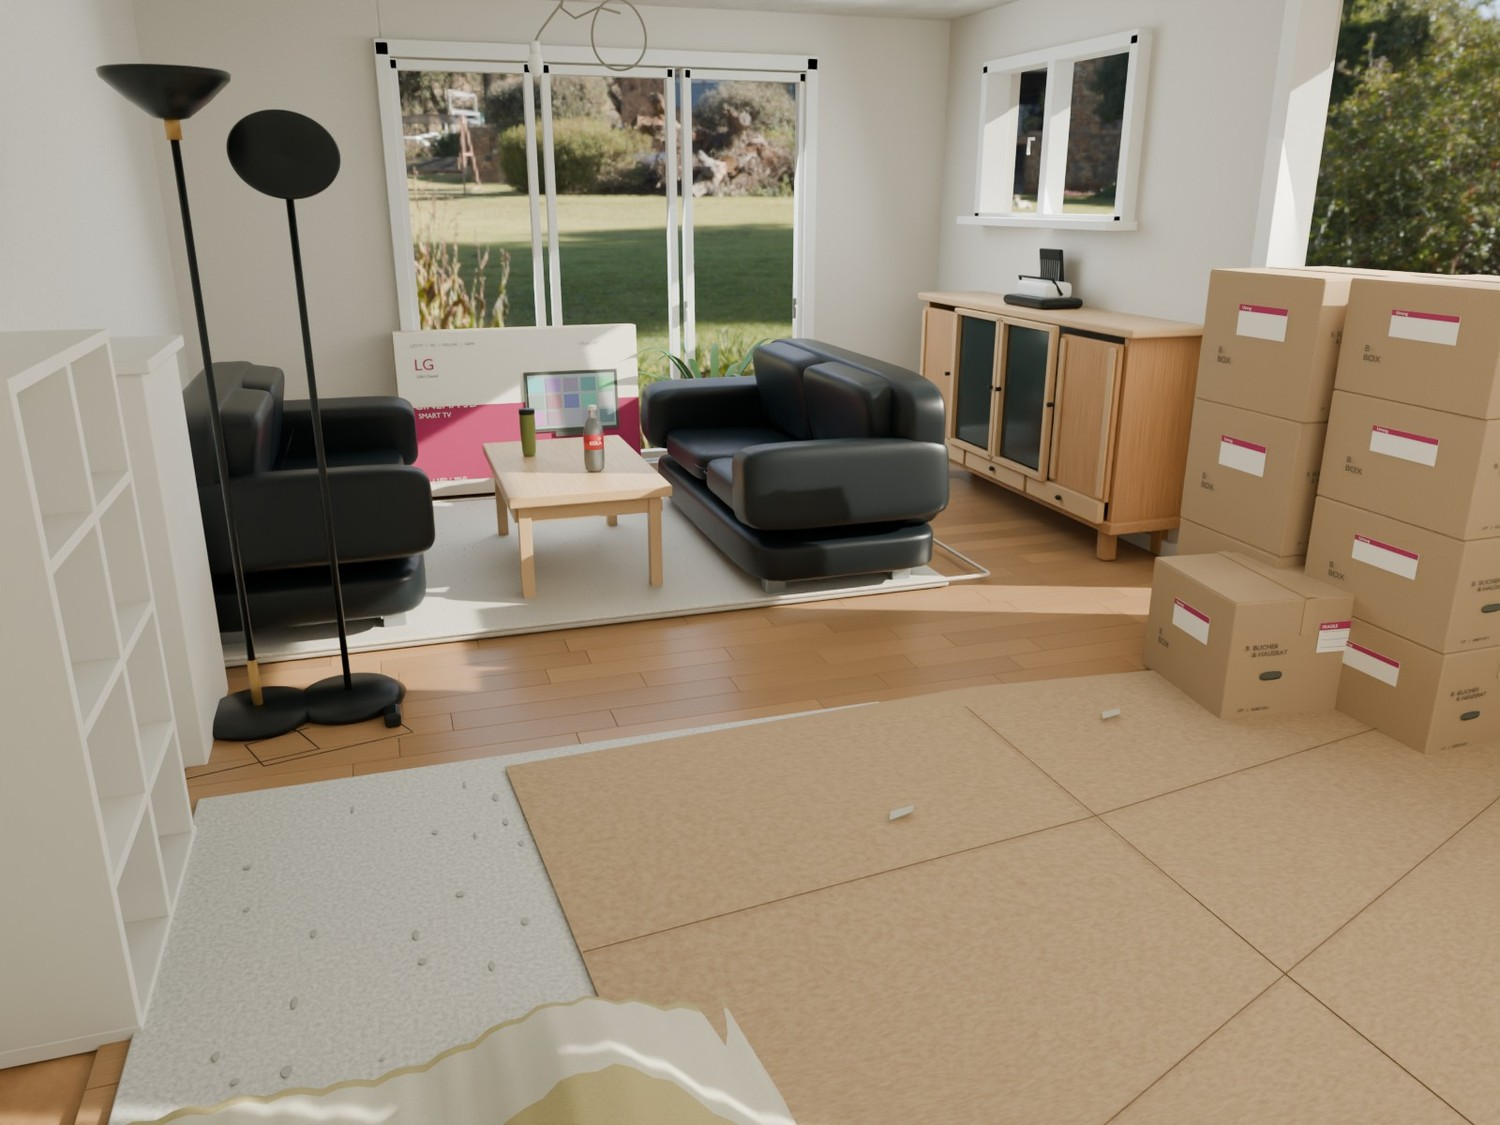
\includegraphics[width=\linewidth]{figures/blender-render.jpg}\par
      \vspace{2mm}
      {\footnotesize Blender render by GPT-6 Astra}
    \end{column}
  \end{columns}
  \vfill
\end{frame}

\begin{frame}{Next steps}
  \begin{itemize}
    \item Literature review
    \item Get detection working
    \item Scene assembly
  \end{itemize}
  \vspace{6mm}
  Goal: an end-to-end baseline (MVP)
\end{frame}

\end{document}
